Sheet metal bending is a process in which bends are formed using a combination of a punch and a die. This process is used to create large number of mechanical products such as furniture panels, shelves, cabinets, housing for electro-mechanical devices etc. \cite{alvaautomated}
The project partner for this thesis \textit{i.e.} \textbf{mech-tron GmbH \& Co. KG} excels in the manufacturing of housing systems for electronic and embedded equipment. In this thesis, manufacturing of one of these sheet metal housing systems will be automated by means of robotic workcell.

\subsection{ASTRO bending cell}
\label{subsec:astro}

\hyperref[acro:AMADA]{AMADA} already offers an automated solution for the bending process in means of a system called ASTRO bending cell. This system consists of a handling robot which can perform production of smaller, complex workpieces and have uniformity in production. However, press brake and the know-how of handling robot come from \hyperref[acro:AMADA]{AMADA}.
The project partner has one of these systems \textit{i.e.} ASTRO-100 II NT HDS 1030 in their production floor. 

The ASTRO-100 II NT cell is an “island solution” that is only available in the HDS-1030 press configuration, ASTRO HP-20 loading and unloading robot, ASTRO-100 II NT bending robot and the external software ASTRO CAM.
The ASTRO-100 II NT cell. \cite{astro100} The production using these system is continous and very fast.

\begin{figure}[h]
    \centering
    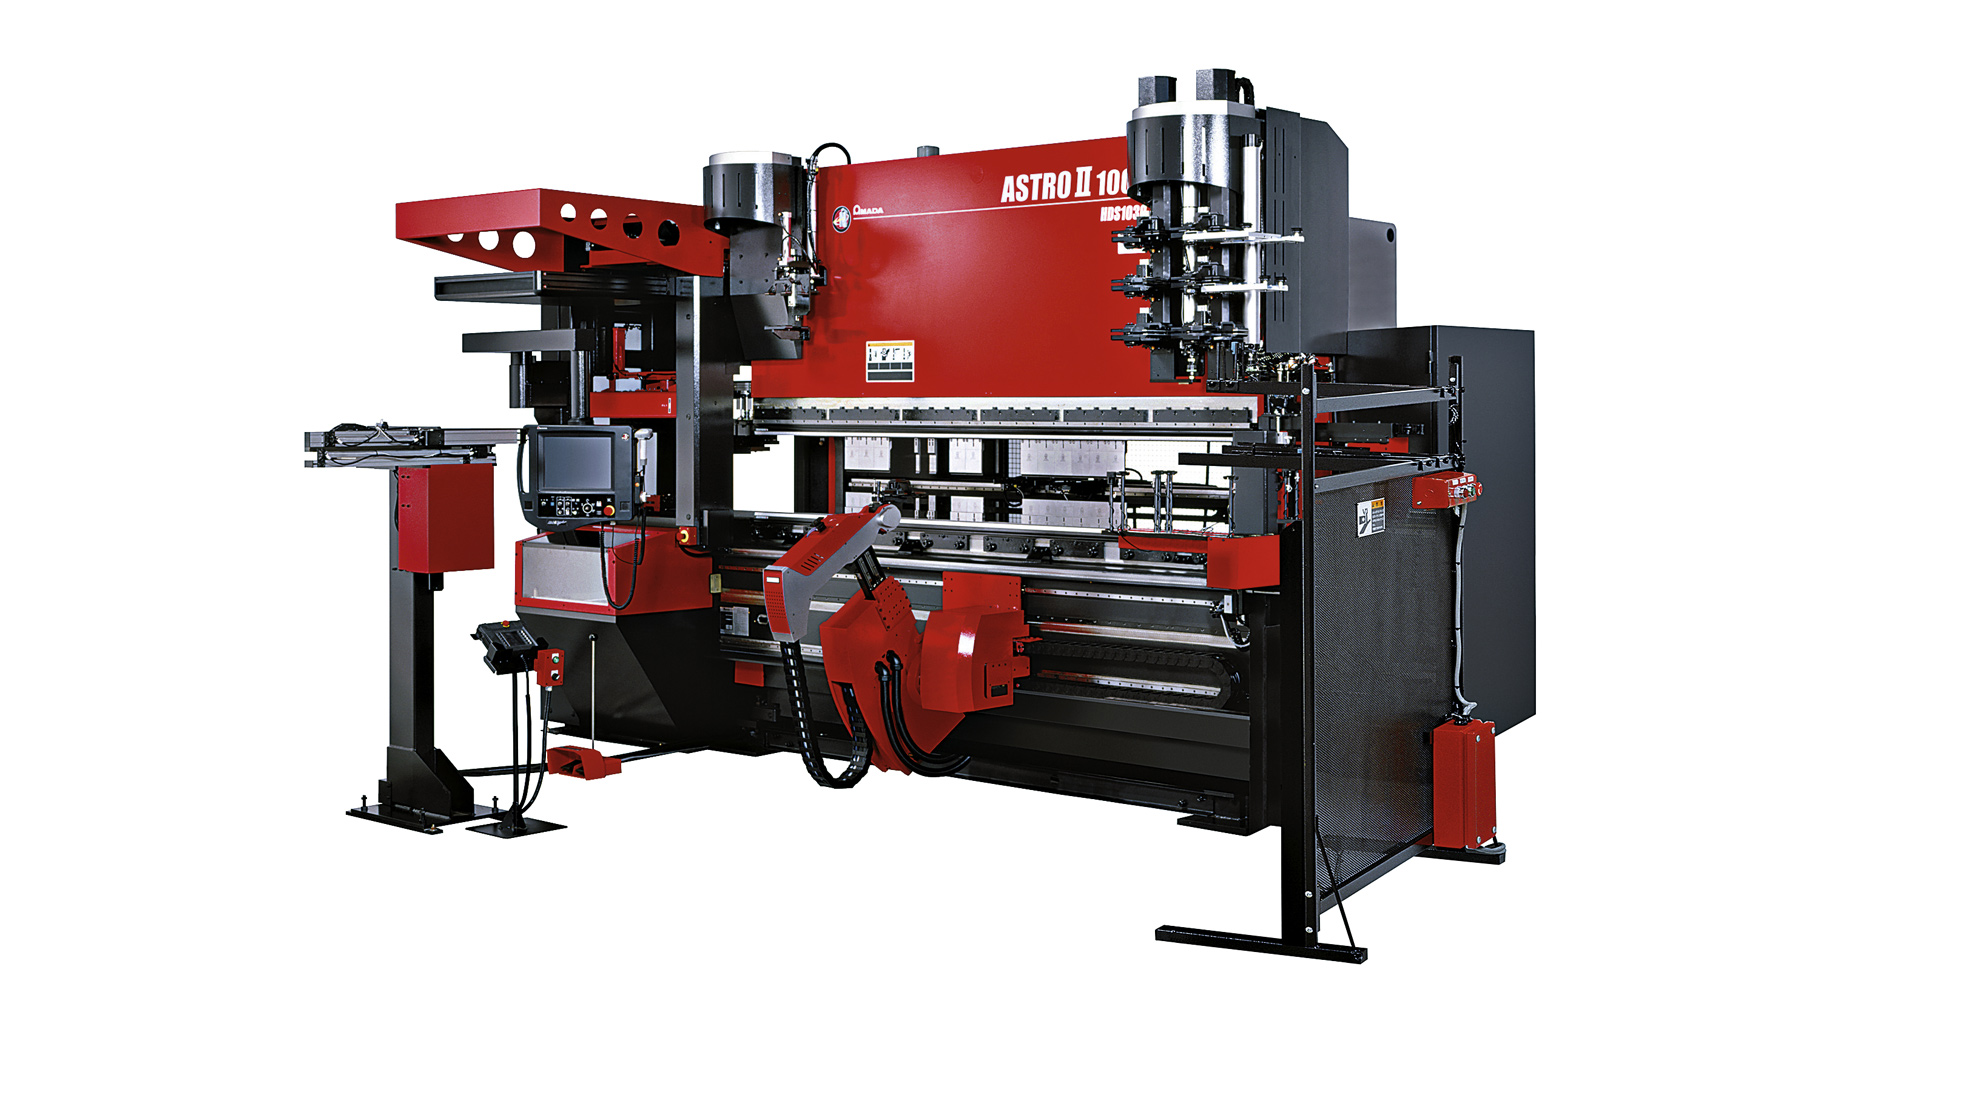
\includegraphics[width=\textwidth]{figures/ASTRO-100.jpg}
    \caption{ASTRO-II 100NT HDS 1030 bending cell. Source: \cite{astro100}}
    \label{fig:astro}
\end{figure}

The main drawback of this system is the software ASTRO-CAM, which is owned by \hyperref[acro:AMADA]{AMADA}, and offers less flexibility and requires support from \hyperref[acro:AMADA]{AMADA} for programming. Without any vision sensors, the system is not smart. It can perform repetitive tasks very fast and with very little interference from operator but without any decision making. Also, the ASTRO robot is non-collaborative and humans cannot work alongside it.
It requires a large area on the production floor which incurs more cost.

In this thesis, this system will be compared to our robotic workcell solution which has collaborative robot and is more cost-effective.

There are various companies in the world which offers automated bending cells. They use industrial robot to bend the parts in the bending machine. \cite{mekoprint, shenchong} However, using a collaborative robot to perform bending tasks is challenging. A collaborative robot generally has low payload capacity and requires better robot motion planning during bending to avoid exceeding joint torques.
In \cite{liu2022metalwiremanipulationplanning}, a cobot is used to collaborate with a bending machine to perform \hyperref[acro:3D]{3D} curving of metal wire and discusses the difficulties in holding the
part in low payload robot gripper during bending and defines the generation of optimum robot motion considering the combined task and motion level constraints.